%!TEX root = ../../../main.tex

\subsection{Existing Technologies}

\acrfull{hpo} is an important step in the machine learning development pipeline. This is usually implemented into other frameworks (as part of a complete pipeline framework). We pay special attention to existing frameworks that are model agnostic, written in \acrfull{python} and are able to treat the objective function as a \textit{black box}.

We also also specify important software tools or protocols used.

\subsubsection{Hyper Parameter Optimization}

Due to the academic nature of the development of \acrshort{hpo} frameworks, there are a plethora of frameworks, with different optimization techniques, goals and interfaces. We present some frameworks and toolkits that introduce specific features or optimization techniques or are industry standard.

\paragraph{Determined} This is an open-source deep learning training platform \parencite{determined-ai}. It allows for distributed training using a custom Horovod-based framework \parencite{alex2018horovod} as well as features to better utilize computational resources (smart scheduling). It's \acrshort{hpo} interface supports ASHA \parencite{li2018massively}, grid search, random search and population-based training. This framework is specifically focused on deep learning, which makes it harder to use with black-box functions.

\paragraph{HpBandSter} This \acrshort{python} package, developed by the AutoML team, implements a distributed HyperBand algorithm, allowing for parallelization of the \acrshort{hpo} \parencite{hpbandster}. It also implements BOHB, which combines bayesian optimization and HyperBand \parencite{pmlr-v80-falkner18a}.

\paragraph{hyperopt} This \acrshort{python} library is intended to be used for serial and parallel \acrshort{hpo} \parencite{hyperopt}. It implements random search and tree parzen estimators. Its parallelization feature can be executed using Apache Spark or MongoDB.

\paragraph{scikit-learn} This framework is one of the most popular frameworks for machine learning in \acrshort{python}. It implements a full development pipeline for machine learning, including \acrshort{hpo} \parencite{scikit-learn}. It implements grid search, random search and successive halving as default available optimization algorithms. It also has community developed add-on algorithms, such as Auto-sklearn \parencite{auto-sklearn} and scikit-optimize \parencite{scikit-optimize}.

\paragraph{Tune} This \acrshort{python} library is part of Ray, an open source framework that provides a simple, universal API for building distributed applications \parencite{ray}. It supports distributed computing and multiple \acrshort{gpu}s per computing node. It implements random search, grid search, a number of bayesian optimization algorithms, Tree-Parzen estimators, HyperBand, gradient-free optimization and BOHB.

\paragraph{Amazon Sagemaker} This cloud \acrshort{machinel} platform, developed by Amazon, is a complete suite of tools for creating, training and deploying \acrshort{machinel} in the cloud \parencite{sagemaker}. This platform implements \acrshort{hpo} algorithms such as random search and bayesian optimization.

\paragraph{Google HyperTune} This training platform is part of Google's AI Platform \parencite{ghypertune}. It supports bayesian optimization, grid search and random search.   

\begin{figure}[hb]
\centering
\begin{tabular}{ccccc}
\subfloat[DeterminedAI]{
\includegraphics[width = 1in]{images/determined.png}} &
\subfloat[AutoML]{
\includegraphics[width = 1in]{images/automl.png}} &
\subfloat[HyperOpt]{
\includegraphics[width = 1in]{images/hyperopt.png}} &
\subfloat[Scikit Learn]{
\includegraphics[width = 1in]{images/scikit.png}} &
\subfloat[Ray Tune]{
\includegraphics[width = 1in]{images/ray_tune.png}} \\
\subfloat[Amazon Sagemaker]{
\includegraphics[width = 0.9in]{images/sagemaker.png}} &
\subfloat[Google HyperTune]{
\includegraphics[width = 0.9in]{images/google_ai.png}}
\end{tabular}
\caption{Hyper Parameter Optimization Libraries}
\end{figure}

\FloatBarrier

\subsubsection{Virtualization}

As a part of the development of the software solution, it was necessary to implement a virtualization mechanism to harmonize the development environment (\acrshort{win}) and the target \acrfull{os} of the Ray framework (Linux). These techniques can be separated on the level at which they operate - hardware virtualization, desktop virtualization and \acrshort{os}-level virtualization. Here we focus our research on \acrshort{os}-level virtualization, as it was at this level (where we are able to run another \acrshort{os}) that the solution was developed on.

\acrshort{os}-level virtualization is a technology that partitions the operating system to create multiple isolated \acrfull{vm} \parencite{10.5555/1571423}.

\paragraph{Chroot} This Unix operation was initially introduced in 1979. Chroot can be considered to be a rudimentary form of virtualization, as it changes the apparent root directory for the current running process and any software running in this environment cannot access files outside the designated root directory, effectively limiting it's access to a directory tree, while still allowing access to other resources \parencite{foundation_2017}.

\paragraph{Docker/Moby} Docker is a set of \acrfull{paas} products that use \acrshort{os}-level virtualization to package software into containers. These tools are open sourced through the Moby Project \parencite{moby_oro}. Docker is one of the most used container runtime engines, with ample documentation, examples and support from the community \parencite[p. 20]{stateofcontainers}.

\paragraph{Kubernetes} This system, also known as \acrshort{k8s}, is an open source system for managing containerized applications across multiple hosts. It provides basic mechanisms for deployment, maintenance, and scaling of applications \parencite{kubernetes}. This system is one of the most used in the industry (both as a self-managed solution as well as prebuilt services such as \acrfull{aks}) \parencite{stateofcontainers}.

\paragraph{VMware Workstation} This virtualization software is one of the most used with regards to hardware level optimization. Although this type of virtualization allows for better control over hardware (allowing for their complete simulation), it increases the overhead of running any software service \parencite{bauer_2019}.

\begin{figure}[hb]
\centering
\begin{tabular}{ccc}
\subfloat[Docker/Moby]{
\includegraphics[width = 1.3in]{images/Moby-logo.png}} &
\subfloat[Kubernetes]{
\includegraphics[width = 1.3in]{images/k8s-logo.png}} &
\subfloat[VMware Workstation]{
\includegraphics[width = 1.3in]{images/vmworkstation.png}}
\end{tabular}
\caption{Commercial Virtualization Products}
\end{figure}

\FloatBarrier

\subsubsection{Machine Learning Data Visualization}

In order to validate the progress and added value that the developed tool provides, it is necessary to verify and validate the \acrshort{hpo} process. For that, we can use data visualization toolkits suited for machine learning purposes, which allow us to verify the training process over time as well as capture data regarding each trial. 

\paragraph{Weights and Biases}

wandb is an open source Python library for experiment tracking, dataset versioning and model management \parencite{wandb}. It also provides graphical tools to plot results, which allows us to analyse the data generated from the training process.

\paragraph{TensorBoard}

This toolkit provides visualization for TensorFlow \parencite{Tensorflow} based projects. It allows for a developer to track and visualize metrics, histograms and more in a intuitive \acrfull{ui}.

\paragraph{Neptune}

This service is a metadata store for \acrshort{machinel}, which allows for experiment tracking and model registering \parencite{neptune}.

\paragraph{Guild AI}

Guild AI is an open source experiment management toolkit, which tracks experiments, automates pipelines and provides data analysis tools for experiment data \parencite{guildai}.

\paragraph{Sacred} 

Sacred is a tool to configure, organize, log and reproduce computational experiments. It is designed to introduce only minimal overhead, while encouraging modularity and configurability of experiments \parencite{klaus_greff-proc-scipy-2017}.

\paragraph{Comet.ml}

Comet.ml enables data scientists and teams to track, compare, explain and optimize experiments and models across the model’s entire lifecycle \parencite{CometML}.

\begin{figure}[hb]
\centering
\begin{tabular}{ccccc}
\subfloat[Weights and Biases]{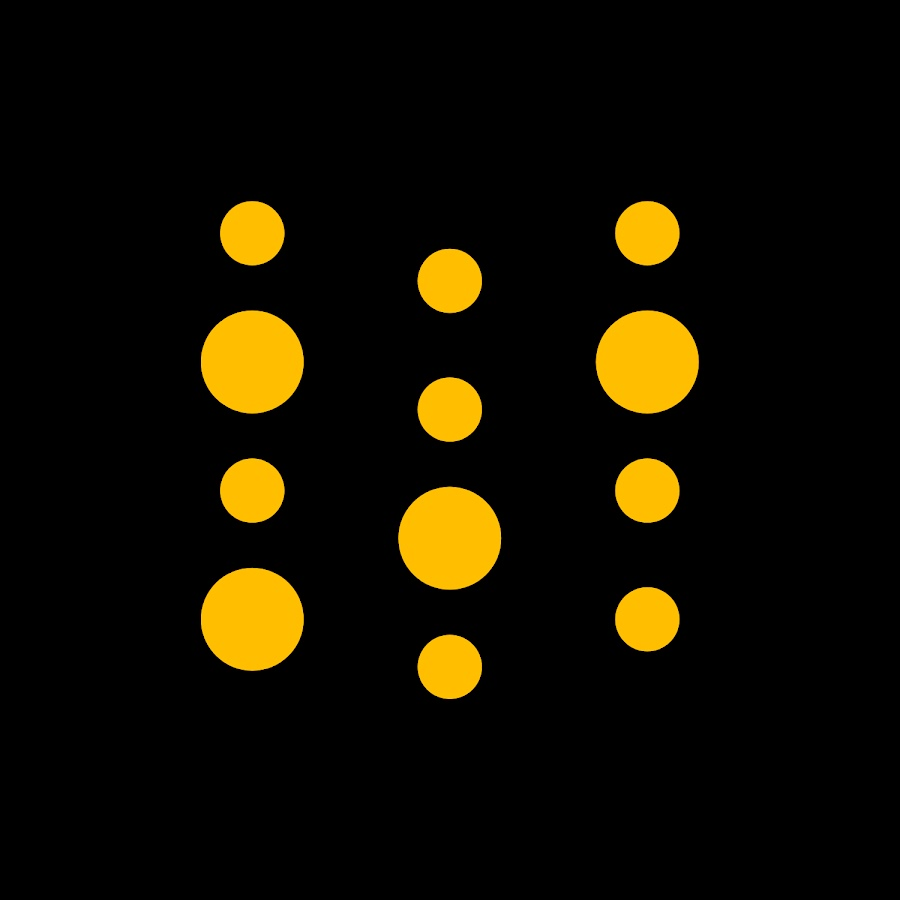
\includegraphics[width = 1in]{images/wandb.png}} &
\subfloat[TensorBoard]{
\includegraphics[width = 1in]{images/tensorboard.png}} &
\subfloat[Neptune]{
\includegraphics[width = 1in]{images/neptune.png}} &
\subfloat[Guild AI]{
\includegraphics[width = 1in]{images/guildai.jpg}} &
\subfloat[Comet]{
\includegraphics[width = 1in]{images/coemt.png}}
\end{tabular}
\caption{Machine Learning Data Visualization Tools}
\end{figure}

\FloatBarrier